% =========================================================================
% AAT — Figure: Strategy DAG with AND/OR and Status Propagation
% Companion to: #def-strategy-dag (Part II Ch.3)
%
% Build:  pdflatex strategy-dag-example.tex
%
% Small worked example showing the AND/OR combination semantics, leaf
% base credences p_v(M_t), edge credences p_ij, and the resulting
% strategy-plan-confidence score P_hat_Sigma = s_{v_root}.
% Worked numerics are visible so the reader can verify propagation.
% =========================================================================
\documentclass[border=10pt]{standalone}
\usepackage{tikz}
\usepackage{amsmath,amssymb}
\usetikzlibrary{arrows.meta,positioning,calc,fit,backgrounds,shapes.geometric}

\begin{document}
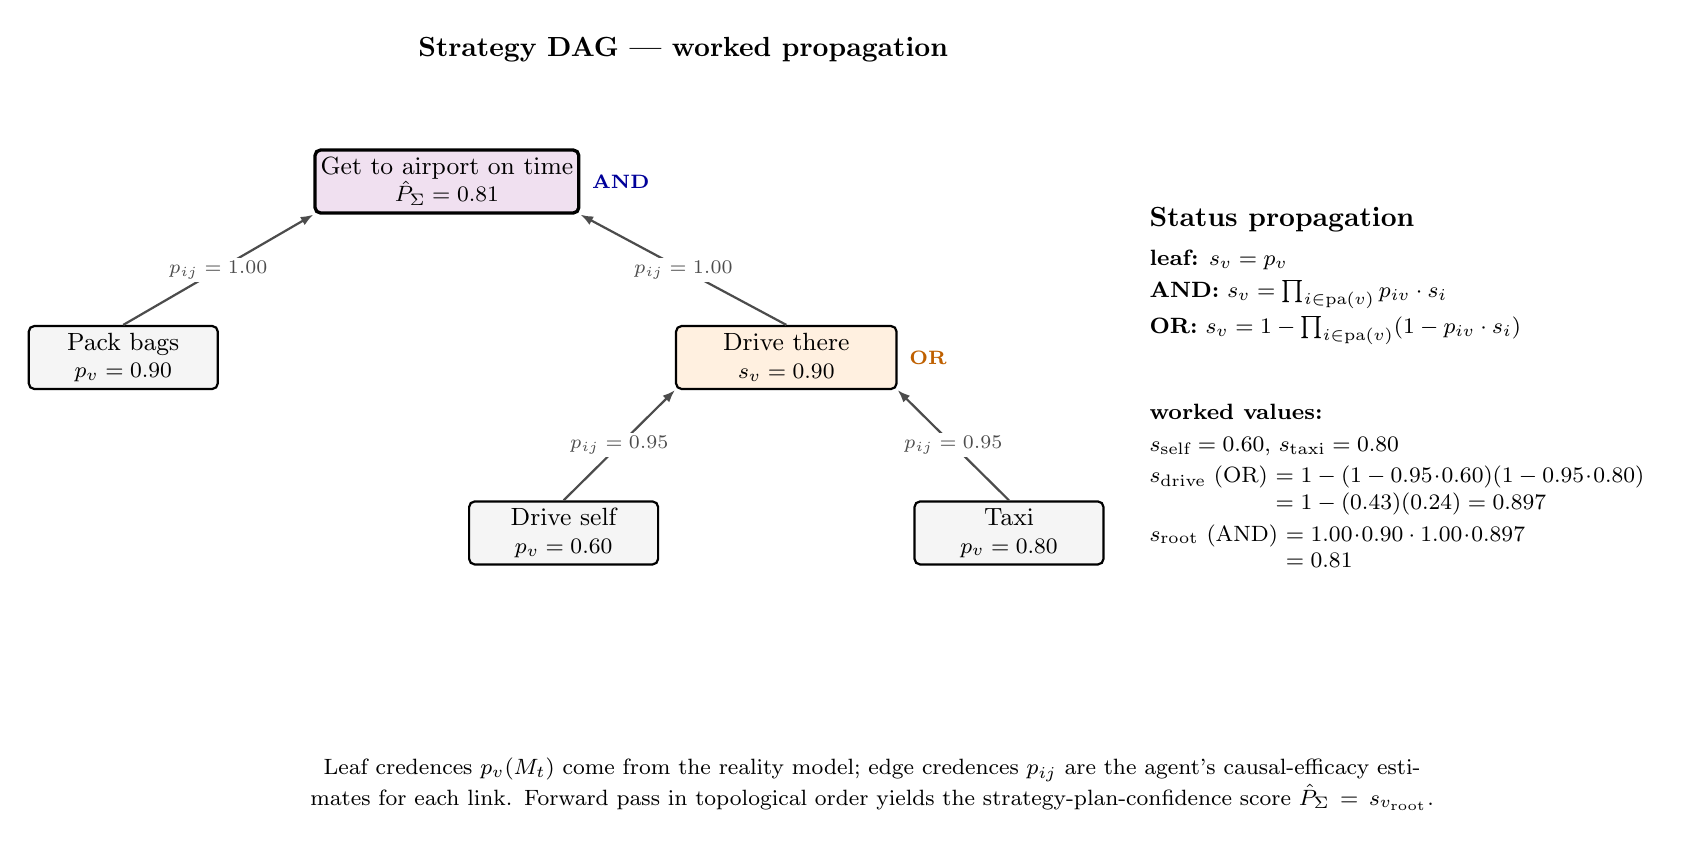
\begin{tikzpicture}[
    font=\small,
    >=Latex,
    node distance=8mm and 14mm,
    % node styles
    root/.style       = {draw, rounded corners=2pt, very thick, fill=violet!12,
                          minimum width=3.2cm, minimum height=8mm, align=center,
                          inner sep=2pt, font=\small},
    andnode/.style    = {draw, rounded corners=2pt, thick, fill=blue!10,
                          minimum width=2.8cm, minimum height=8mm, align=center,
                          inner sep=2pt, font=\small},
    ornode/.style     = {draw, rounded corners=2pt, thick, fill=orange!12,
                          minimum width=2.8cm, minimum height=8mm, align=center,
                          inner sep=2pt, font=\small},
    leaf/.style       = {draw, rounded corners=2pt, thick, fill=gray!8,
                          minimum width=2.4cm, minimum height=8mm, align=center,
                          inner sep=2pt, font=\small},
    % gate tags
    gate/.style       = {font=\scriptsize\bfseries, inner sep=1pt},
    andgate/.style    = {gate, blue!60!black},
    orgate/.style     = {gate, orange!75!black},
    % edges
    sedge/.style      = {-{Latex[length=1.6mm]}, thick, black!70},
    elabel/.style     = {font=\scriptsize, fill=white, inner sep=1pt,
                          midway, sloped=false}
  ]

% ============================================================
% Layout (top-down). Root at top, leaves at bottom.
% ============================================================

% Root (AND of two sub-goals)
\node[root] (root)
  {Get to airport on time \\[-1pt] {\footnotesize $\hat P_\Sigma = 0.81$}};
\node[andgate, anchor=west] at ($(root.east) + (3pt, 0)$) {AND};

% Two children of root
\node[leaf, below left=14mm and 12mm of root] (pack)
  {Pack bags \\[-1pt] {\footnotesize $p_v = 0.90$}};
\node[ornode, below right=14mm and 12mm of root] (drive)
  {Drive there \\[-1pt] {\footnotesize $s_v = 0.90$}};
\node[orgate, anchor=west] at ($(drive.east) + (3pt, 0)$) {OR};

% Two children of drive (OR)
\node[leaf, below left=14mm and 2mm of drive] (self)
  {Drive self \\[-1pt] {\footnotesize $p_v = 0.60$}};
\node[leaf, below right=14mm and 2mm of drive] (taxi)
  {Taxi \\[-1pt] {\footnotesize $p_v = 0.80$}};

% Edges with credences (p_ij)
\draw[sedge] (pack.north)  -- node[elabel] {$p_{ij}=1.00$} (root.south west);
\draw[sedge] (drive.north) -- node[elabel] {$p_{ij}=1.00$} (root.south east);
\draw[sedge] (self.north)  -- node[elabel] {$p_{ij}=0.95$} (drive.south west);
\draw[sedge] (taxi.north)  -- node[elabel] {$p_{ij}=0.95$} (drive.south east);

% ============================================================
% Propagation legend / key (right side)
% ============================================================
\begin{scope}[xshift=8.8cm, yshift=-0.2cm]
  \node[anchor=north west, font=\bfseries] (keyhdr) at (0, 0)
    {Status propagation};

  \node[anchor=north west, font=\footnotesize, align=left]
    at (0, -0.55) (form)
    {
      \textbf{leaf:} $s_v = p_v$ \\[2pt]
      \textbf{AND:} $s_v = \prod_{i\in\text{pa}(v)} p_{iv} \cdot s_i$ \\[2pt]
      \textbf{OR:} $s_v = 1 - \prod_{i\in\text{pa}(v)} (1 - p_{iv}\cdot s_i)$
    };

  \node[anchor=north west, font=\footnotesize, align=left]
    at (0, -2.5) (calc)
    {
      \textbf{worked values:} \\[2pt]
      $s_{\text{self}} = 0.60$, $s_{\text{taxi}} = 0.80$ \\[2pt]
      $s_{\text{drive}}$ (OR) $= 1 - (1-0.95\!\cdot\!0.60)(1-0.95\!\cdot\!0.80)$\\
      \phantom{$s_{\text{drive}}$ (OR) }$= 1 - (0.43)(0.24) = 0.897$ \\[2pt]
      $s_{\text{root}}$ (AND) $= 1.00\!\cdot\!0.90 \cdot 1.00\!\cdot\!0.897$\\
      \phantom{$s_{\text{root}}$ (AND) }$= 0.81$
    };
\end{scope}

% ============================================================
% Title and caption
% ============================================================
\node[font=\bfseries, anchor=south] at (3.0, 1.4)
  {Strategy DAG --- worked propagation};
\node[font=\footnotesize, anchor=north, text width=15cm, align=center]
  at (5.4, -7.2)
  {Leaf credences $p_v(M_t)$ come from the reality model; edge credences $p_{ij}$
   are the agent's causal-efficacy estimates for each link. Forward pass in
   topological order yields the strategy-plan-confidence score
   $\hat P_\Sigma = s_{v_{\text{root}}}$.};

\end{tikzpicture}
\end{document}
